%
% drei.tex
%
% (c) 2018 Prof Dr Andreas Müller, Hochschule Rapperswil
%
\documentclass[tikz]{standalone}
\usepackage{times}
\usepackage{amsmath}
\usepackage{txfonts}
\usepackage[utf8]{inputenc}
\usepackage{graphics}
\usetikzlibrary{arrows,intersections}
\usetikzlibrary{math}
\begin{document}
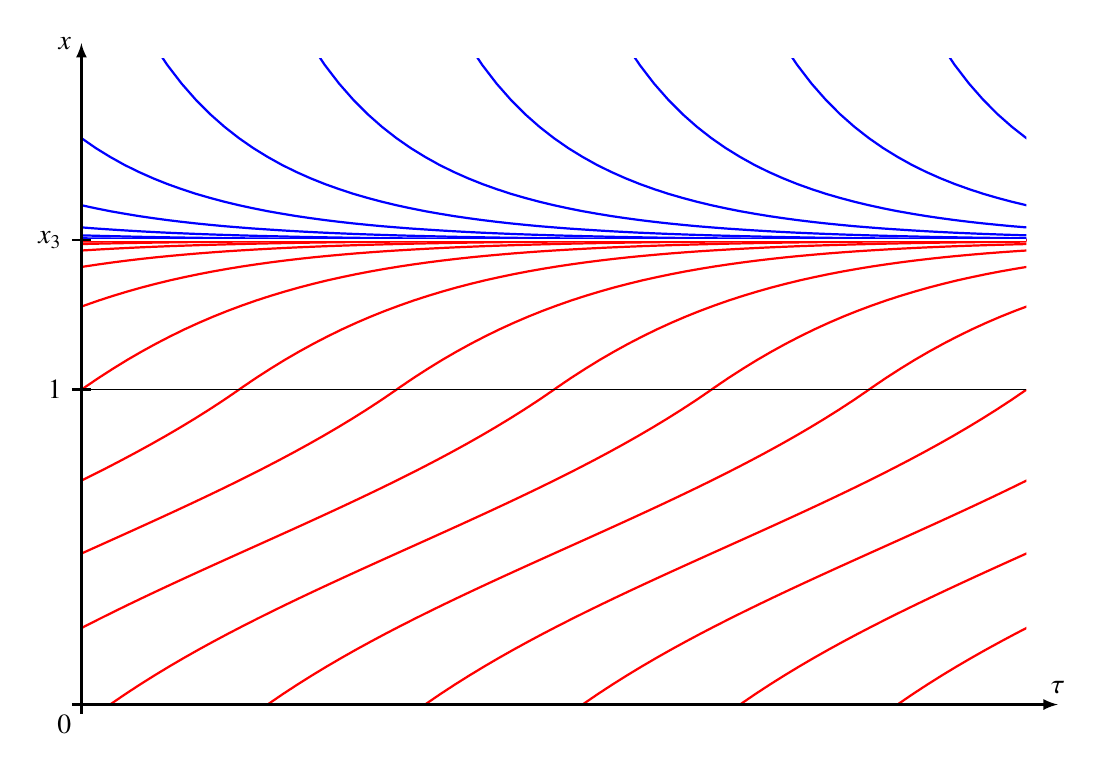
\begin{tikzpicture}[thick, >= latex, scale=4]

\tikzmath{
	real \l;
	\l = 0.7;
	real \a, \b;
	\a = sqrt(\l - 0.25);
	\b = sqrt(0.25 + \l);
	real \xthree;
	\xthree = 0.5 + \b;
	real	\taua, \taub, \z;
	\taua = (3.1415/180) * atan(1/(2*\a)) / \a;
	\z = 1/(2*\b);
	\taub = 0.5 * ln((1+\z)/(1-\z)) / \b;
}

\begin{scope}
	\clip (0,1) rectangle (3,2.05);
	\foreach\translate in {-8,-7,...,4}{
		\draw[color=blue,domain=0.5:5,samples=100]
			plot ({\x+\translate/2},{0.5 + \b/tanh(\b*\x)});
	}
\end{scope}

\begin{scope}
	\clip (0,1) rectangle (3,2.05);
	\foreach\translate in {-6,-5,...,5}{
		\draw[color=red,domain=0.5:5,samples=100]
			plot ({\x+\translate/2-\taub},{0.5 + \b*tanh(\b*\x))});
	}
\end{scope}

\begin{scope}
	\clip (0,0) rectangle (3,1);
	\foreach\translate in {0,1,...,9}{
		\draw[color=red,domain=-2.3:2.3,samples=100]
			plot ({\x+\translate/2-\taua},{0.5 + \a * tan(\a * \x r)});
	}
\end{scope}

\draw[->] (-0.03,0)--(3.1,0) coordinate[label={$\tau$}];
\draw[->] (0,-0.03)--(0,2.1) coordinate[label={left:$x$}];

\node at (0,0) [below left] {$0$};

\draw[color=white] (0,{\xthree})--(3.0,{\xthree});

\draw[line width=0.5] (0,1)--(3,1);
\draw (-0.03,1)--(0.03,1);
\node at (-0.03,1) [left] {$1$};

\draw (-0.03,{\xthree})--(0.03,{\xthree});
\node at (-0.03,{\xthree}) [left] {$x_3$};

\end{tikzpicture}
\end{document}

